\documentclass[11pt,a4paper]{moderncv}

\usepackage[english]{babel}
\usepackage[utf8]{inputenc}
\usepackage{multicol}
\moderncvtheme[red]{casual}
\usepackage{moderncv-additions}

% adjust the page margins
\usepackage[scale=0.8]{geometry}
\setlength{\hintscolumnwidth}{3cm}

\AtBeginDocument{\recomputelengths}

% personal data
\firstname{Philipp}
\familyname{Scholl}
\address{%
    5 Merchants Place, Stephen Street}{%
    W91 C3Y6, Dunlavin, Co. Wicklow}%
\mobile{+353 87 1922755}
\email{rayleighsjeans@gmail.com}
\photo[64pt]{picture}

% \title{Resumé title (optional)}
% \phone{phone (optional)}
% \fax{fax (optional)}
% \extrainfo{additional information (optional)}

% \nopagenumbers{}
% uncomment to suppress automatic page numbering for CVs
% longer than one page

\newcommand{\sign}[1]{%
  \begin{tabular}[t]{@{}l@{}}
  \makebox[1.5in]{\dotfill}\\
  \strut\emph{#1}\strut%
  \end{tabular}}%
\newcommand{\position}{%
    Softwareentwickler Windows (w/m/d)}%
\newcommand{\posaddress}{%
    Thermo Fisher Scientific Inc.\\%
    Personalstelle, Ref.: 133730BR\\%
    Germering, Germany}%

% content
\begin{document}
%
% color redefinitions must be after \begin{document}
% \definecolor{firstnamecolor}{RGB}{138,74,57}%
\definecolor{firstnamecolor}{RGB}{0,50,95}%
\definecolor{familynamecolor}{RGB}{0,50,95}%
\definecolor{quotecolor}{RGB}{0,70,110}%
\definecolor{addresscolor}{RGB}{0,70,110}%
\definecolor{sectionrectanglecolor}{RGB}{0,50,95}%
\definecolor{sectiontitlecolor}{RGB}{0,50,95}%
\definecolor{subsectioncolor}{RGB}{0,70,110}%
\definecolor{footersymbolcolor}{RGB}{0,70,110}%
%
\makeatletter%
\pagestyle{empty}%
\chapter*{Application}{~Form}%
%
\vspace*{3.5cm}%
\begin{minipage}{\textwidth}%
    \vspace*{30mm}%
    \familynamestyle{\@firstname}~\firstnamestyle{\@familyname}%
    \hspace*{10mm}%
    {{\color{firstnamecolor}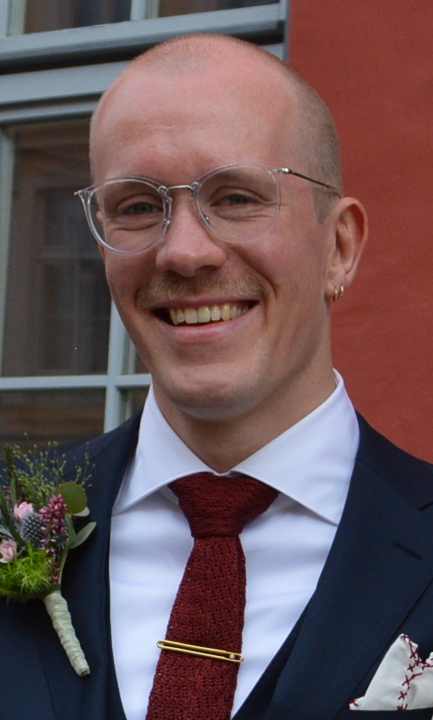
\includegraphics[width=96pt]{%
                    ../figures/images/52.png}}}\\[0.3cm]
    \@addressstreet\\[0.0cm]%
    \@addresscity\\[0.3cm]%
    \mobilesymbol~\@mobile\\[0.3cm]%
    \emailsymbol~\@email%
\end{minipage}%
\begin{minipage}{70pt}%
\end{minipage}%
\vfill%
%
% letter
\newpage%
\makeatletter%
\pagestyle{fancy}%
\chapter{Curriculum}{~Vitae}%
\makequote%


\section{Personal~Information}
\cvline{Name}{\@firstname~\@familyname}
\cvline{Address}{\@addressstreet\newline\@addresscity, Ireland}
\cvline{Telephone}{\@mobile}
\cvline{eMail}{\@email}
\cvline{Date~of~Birth}{15th~of~June~1994~in~Demmin}
\cvline{Nationality}{Germany}
\cvline{Family~Status}{married}
\cvline{Sex}{Male}
\makeatother

\section{Languages}
\cvline{German}{first language, mother tongue}{}
\cvline{English}{second language, first foreign lingo, C2 certificate\newline 7 years of school education}{}
\cvline{Russian}{third language, second foreign lingo\newline 5 years of school education}{}

% \section{School}
% \cventry{08/2000~--~03/2004}{Elementary~School}{Grundschule~Jarmen\newline~Jarmen}{}{}{}
% \cventry{08/2004~--~08/2010}{Middle~School}{Regionale~Schule~Jarmen\newline~Jarmen}{}{}{}
% \cventry{08/2010~--~06/2012}{Academic~High~School}{%
%     Schlossgymnasium Gützkow,~Gützkow\newline}{}%
% {Higher~Education~Entrance~Qualification\newline}{%
%     (Certificate~included)}

\section{Higher Education}
\cventry{10/2012~--~09/2015}{Bachelors~Degree~in~Physics}{Ernst-Moritz-Arndt~University}
{Greifswald}{Bachelor~of~Sciences}{}
\cventry{10/2012~--~10/2017}{Master’s~Degree~in~Physics}{%
    Ernst-Moritz-Arndt~University}%
{Greifswald}{Master~of~Sciences}{}
\cventry{11/2017~--~now}{Doctor~of~Philosophy~-~Physics}{%
    Max-Planck~Institute~for~Plasma~Physics}%
{Greifswald}{Thesis submitted, defense pending}{}

\section{Professional Experience}
\cventry{07/2021~--~04/2024}{Software~Developer - C/C++}{%
    Krauss-Maffei Wegmann Nexter Defense Systems}%
{Munich}{Advanced C/C++, embedded development, frameworks, APIs, AI, computer generated forces, dynamics \& simulator logic}{}%
\cventry{11/2017~--~05/2021}{Researcher/Scientist, Ph.D. - Plasma Fusion}{%
    Max-Planck~Institute~for~Plasma~Physics}%
{Greifswald}{Project management, large scale data analysis, science, modelling, simulation, embedded development, international collaboration, professional documentation}{}

\subsection{Additional Training}
\cventry{02/2022}{Advanced C++ (for Embedded Systems)}{%
    MicroConsult Microelectronics Consulting \& Training GmbH}%
{Munich}{basics, patterns, idioms, paradigms, `modern style' C++}{}
\cventry{Jun.~2019}{Plan,~Motivate,~Achieve:~Time~and~Self-Management}{Transferable~Skills~Seminar}{R.~Thompson}{International~Helmholtz~Graduate~School~for~Plasma~Physics}{}
\cventry{Jun.~2019}{Presentation~Skill~Workshop}{Transferable~Skills~Seminar}{B.~Hey}{International~Helmholtz~Graduate~School~for~Plasma~Physics}{}

\section{Technical \& Software Development Experience}
\cventry{2021-24}{Software Engineering}{Krauss-Maffei Wegmann; Software
Architecture \& Components}{Munich}{advanced C/C++; Scrum/agile development and design; extended unit, component and regression testing; embedded development; (physics) simulation and AI; CI/CD, Jira, Git/SVN; CMake \& CTest/GTest; Havok Engine \& Unreal Engine 5; GTC 2023 attendance}{}
\cventry{2017-21}{Data Acquisition Development}{Max-Planck Institute for Plasma physics}{Greifswald}{embedded C/C++ development for data acquisition, LabVIEW; data center API for research purposes; Python: large scale data generation, modelling, evaluation and visualization, stereoscopic tomography and simulation; IDL \& Fortran; Git; documentation and presentation of technical content}{}
\cventry{2016-17}{HPC C/C++ Particle-In-Cell Simulation}{Ernst-Moritz-Arndt University; Computational Sciences}{Greifswald}{HPC C/C++ development for particle physics simulation of low-temperature gaseous discharges; Open/MPI \& Slurm; multithreading}{}
\cventry{2016}{Neural Networks and Large Linear Optimizations}{Ernst-Moritz-Arndt University; Advanced Numerics}{Greifswald}{introduction to and development of neural networks, MATLAB}{}
\cventry{2015}{Stereoscopic Particle Tracking and Video Processing}{Ernst-Moritz-Arndt University; Complex Plasmas}{Greifswald}{multi-camera system video analysis, stereoscopic 3D tracking of microscopic particles; development and construction of in-situ microelectronics; MATLAB}{}
\cventry{2012-15}{Computational Sciences}{Ernst-Moritz-Arndt University}{Greifswald}{C/C\# numerical simulation (electrostatic Poisson); Linux development; Assembler programming for custom built electronics}{}


% \section{Research Experience}
% \cventry{11/2017~--~now}{PhD:~`Impurity~radiation~and~transport~at~the~stellarator~Wendelstein~7-X'}{Division~of~Stellarator~Dynamics~and~Transport,~Prof.~Dr.~T.~Klinger\newline}{}{Max-Planck~Institute~for~Plasma~Physics,~Greifswald\newline}{real~time~feedback~on~plasma~radiation,~evaluation~of~local~radiation~sensitivity, Python \& LabVIEW (C++) embedded software development}
% \cventry{11/2017~--~05/2021}{International~Helmholtz~Graduate~School~for~Plasma~Physics}
% {Graduate~School~for~Doctoral~Candidates~at~the~MPI~for~Plasma Physics\newline}{}{MPI~for~Plasma~Physics,~Greifswald;~University~of~Greifswald\newline}{presentations~and~participation~in~colloquia,~workshops~and~conferences}
% \cventry{10/2016~--~10/2017}{Master~Thesis:~`Kinetic~Effects~in~RF~Discharges'}{Research~Group~of~Prof.~Dr.~Ralf~Schneider\newline}{}{Institute~of~Physics,~University~of~Greifswald\newline}{C/C++ particle simulation code development - C++ 2d3v PIC simulation of ccrf discharges}
% \cventry{04/2016~--~10/2016}{Research~Group~Internship}{`Electric~field~strength~spectroscopy~in~dielectric~barrier~discharges'\newline}{}{Research~Group~of~Prof.~Dr.~Jürgen~Meichsner\newline}{Institute~of~Physics,~University~of~Greifswald}
% % \cventry{10/2015~--~04/2016}{Advanced Practical Laboratory Course}{Advanced experimental methodology\newline}{}{Institute~of~Physics,~University~Greifswald}{}
% \cventry{10/2015~--~07/2016}{Intership~in~the~Group~of~Prof.~Dr.~Melzer}{Complex~Plasma~Systems,~Experiment~Setup\newline}{}{Institute~of~Physics,~University~of~Greifswald}{}
% \cventry{05/2015~--~09/2015}{Bachelor~Thesis:~`Modenanregung~in~Yukawa-Bällen'}{Research~Group~of~Prof.~Dr.~Andre~Melzer\newline}{}{University~of~Greifswald\newline}{Stereoscopic particle diagnostics with MATLAB}
% \cventry{10/2012~--~04/2014}{Basic~Practical~Laboratory~Course}{Basic~experiments~in~all~research~fields~at~the~Institute~of~Physics\newline}{}{University~of~Greifswald}{}

% \section{Lecturing Experiences}
% \cventry{2014~--~2018}{Assistant~Associate~in~the~Practical~Course~-~Physics}{in:~Study~Programme~of~Humane~Medicine\newline}{}{Institute~of~Physics,~University~of~Greifswald}{}

% \section{Publications (Excerpt)}
% \cventry{May~2018}{`PIC~Simulation~of~electronegative~CCRF~discharges'}{Authors:~P.~Matthias,~R.~Schneider,~J.~Meichsner,~G.~Bandelow,~J.~Duras,~K.~Matyash, K.-F.~Lüskow,~D.~Kahnfeld,~S.~Kemnitz,~L.~Lewerentz~and~P.~Hacker}{    doi:~10.1140/epjd/e2017-80565-y}{}{}
% \cventry{Dec.~2019}{`Measurement of edge ion temperature in W7-X with island divertor by retarding field analyzer'}{Authors:~Y.~Li,~T.~Henkel,~Y.~Liang,~A.~Knieps,~P.~Drews,~C.~Killer,~D.~Nicolai,~J.~Cosfeld,~J.~Geiger,~Y.~Feng,~F.~Effenberg,~D.~Zhang,~P.~Hacker,~D.~Höschen,~G.~Satheeswaran,~S.~Liu,~O.~Grulke,~M. Jakubowski, S.~Brezinsek,~M.~Otte,~O.~Neubauer,~B.~Schweer1,~G.~S.~Xu,~J.~Cai,~Z. Huang, and the W7-X~Team}{doi:~10.1088/1741-4326/ab3a79}{}{}
% \cventry{Jul.~2019}{`The~influence~of~impurity~radiation~locations~on~the~plasma~performance~in~stellarator~Wendelstein~7-X'}{Authors:~D.~Zhang,~R.~Burhenn,~F.~Reimold,~P.~Hacker,~L.~Giannone,~K.~J.~Brunner,~B.~Buttenschön,~G.~Fuchert,~H.~P.~Laqua,~K.~Rahbarnia,~C.~D.~Beidler,~S.~Brezinsek,~Y.~Feng,~M.~Jakubowski,~R.~König}{}{}{}
% \cventry{Feb.~2020}{`Absence~of~Non-Local~Electron~Heat~Transport~in~ASDEX~Upgrade~and~Wendelstein~7-X~and~Modelling~with~the~Transport~Code~ASTRA'}{Authors:~K.~Höfler,~T.~Happel,~P.~Hennequin,~U.~Höfel,~F.~Ryter,~U.~Stroth,~A.~Bock,~P.~David,~S.~Denk,~A.~Dinklage,~G.~Fuchert,~P.~Hacker,~M.~Hirsch,~P.~A.~Schneider,~J.~Schilling,~T.~Stange,~G.~Tardini,~T.~Andreeva,~M.~Beurskens,~S.~Bozhenkov,~K.~J.~Brunner,~N.~Chaudhary,~H.~Damm,~U.~Neuner,~J.~W.~Oosterbeek,~E.~Pasch,~K.~Rahbarnia,~H.~Thomsen, M.~Zanini,~D.~Zhang,~the~ASDEX~Upgrade~Team,~the~Wendelstein~7-X~Team}{}{}{}
% \cventry{Sep.~2020}{`Stellarator-Tokamak~Energy~Confinement~Comparison~based~on~ASDEX~Upgrade~and~Wendelstein~7-X~Hydrogen~Plasmas'}{Authors:~U.~Stroth,~G.~Fuchert,~M.~N.A.~Beurskens,~G.~Birkenmeier,~P.~Schneider,~E.R.~Scott,~K.J.~Brunner,~F.~Günzkofer,~P.~Hacker,~O.~Kardaun,~J.~Knauer,~K.~Rahbarnia,~D.~Zhang}{doi:~0.1088/1741-4326/abbc4a}{}{}
% \cventry{Jan.~2023}{`First feedback-controlled divertor detachment in W7-X: Experience from TDU operation, prospects for operation with actively cooled divertor'}{Authors:~M. Krychowiak, R. König, T. Barbui, S. Brezinsek, J. Brunner, F. Effenberg, M. Endler, Y. Feng, E. Flom, Y. Gao, D. Gradic, P. Hacker, J.H. Harris, M. Hirsch, U. Höfel, M. Jakubowski, P. Kornejew, M. Otte, A. Pandey, T.S. Pedersen, A. Puig, F. Reimold, O. Schmitz, T. Schröder, V. Winters, D. Zhang}{doi:~10.1016/j.nme.2023.101363}{}{}
% \cventry{Sep.~2021}{`Plasma radiation behavior approaching high-radiation scenarios in W7-X'}{Authors:~D. Zhang, R. Burhenn, Y. Feng, R. König, B. Buttenschön, C.D. Beidler, P. Hacker, F. Reimold, H. Thomsen, R. Laube, T. Klinger, [\dots],  the W7-X Team}{doi:~10.1088/1741-4326/ac2b75}{}{}
% \cventry{Oct.~2021}{`2D measurements of parallel counter-streaming flows in the W7-X scrape-off layer for attached, detached plasmas'}{Authors:~V. Perseo, V. Winters, Y. Feng, F. Reimold, O.P. Ford, R. König, S.A. Bozhenkov, K.J. Brunner, R. Burhenn, P. Drewelow, D.A. Ennis, Y. Gao, D. Gradic, P. Hacker [\dots]and the W7-X Team}{doi:~10.1088/1741-4326/ac277a}{}{}%
% \cventry{Oct.~2021}{`Bolometer tomography on W7-X for study of radiation asymmetry'}{Authors:~D. Zhang, R. Burhenn, C.D. Beidler, Y. Feng, H. Thomsen, C. Brandt, S. Buller, F. Reimold, P. Hacker [\dots]and the W7-X Team}{doi:~10.1088/1741-4326/ac2778}{}{}
% \cventry{Jul.~2020}{`Large wetted areas of divertor power loads at Wendelstein 7-X'}{Authors:~H. Niemann, P. Drewelow, M. W. Jakubowski, A. Puig Sitjes, B. Cannas, Y. Gao, F. Pisano, R. König, R. Burhenn, P. Hacker, F. Reimold, D. Zhang, K. J. Brunner, J. Knauer, T. Sunn Pedersen and the W7-X Team}{doi:~10.1088/1741-4326/ab937a}{}{}

% \section{Research Interests}
% \cvline{}{plasmaphysics,~low-temperature~plasmaphysics,\newline%
%     ~high-temperature~plasmaphysics,~numerical~simulation,~computational~science,\newline
%     ~diagnostics,~data~evaluation,~machine~learning,~diagnostic~control}

% \section{Extra-Curriculars \& Extramural Activities}
% \cventry{2007~--~2010}{Participation~in~the\newline`Baltic~Sea~School~Exchange~Program'}{Finnvedens~Gymnasium~`Figy';~Värnamo,~Sweden}{}{}{}
% \cventry{2011}{Qualification~for~the~German~Dragon~Boat~National~Team~`Junior~A'}{Participation~in~the~10th~IDBF~World~Dragon~Boat~Racing~Championships\newline}{}{Tampa~Bay,~FL;~United~States~of~America\newline}{9~Gold~Medals,~2~Silver~Medals}
% \cventry{2012}{Entering~of~the~`Hochschul-Sportgemeinschaft~Greifswald~e.V'}{Department~of~Canoe/Dragonboat\newline2015-2016~Trainer~of~the~Dragon~Boat~Team~`Greifendrachen'}{}{}{}{}
% \cventry{2017}{Qualification~for~the~German~Dragon~Boat~National~Team~`U24'}{Participation~in~the~13th~IDBF~World~Nations~Championships\newline}{}{Divonne-Les-Baines,~France}{}
% \cventry{2021~--~now}{(Olympic)~Weightlifting~Team~Participation\newline    ESV~München~Neuaubing~--~Local~League~and~Individual~Competitions}{County~Oberbayern~and~Bavarian~League~2021/22,~22/23,~23/24\newline}{}{1st place Munich Championships '23, 2nd place Oberbayern Championships '23}{}%


%\subsection{Conferences \& Workshops}
% \cventry{May~2019}{Consistently~calculating~the~radiated~power~in~near~real~time~at~the~stellarator~Wendelstein~7-X}{P.~Hacker,~F. Reimold,~D.~Zhang,~M.~Krychowiak,~R.~Burhenn,~T.~Klinger}{DPG-Frühjahrstagung~der~Sektion~Materie~und~Kosmos~(SMuK),~Munich,~Germany,~2019}{}{}
% \cventry{May~2019}{Plasma~Terminating~Events~in~Large~Stellarators}{D.~Maier,~A.~Dinklage,~J.~Baldzuhn,~R.~Burhenn,~R.~Bussiahn,~B.~Buttenschön,~P.~Hacker, [...],~the~W7-X~Team}{DPG-Frühjahrstagung~der~Sektion~Materie~und~Kosmos~(SMuK),~Munich,~Germany,~2019}{}{}
% \cventry{Jul.~2019}{The~influence~of~impurity~radiation~locations~on~the~plasma~performance~in~stellarator~Wendelstein~7-X}{D.~Zhang,~R.~Burhenn,~F.~Reimold,~P.~Hacker, [...],~the~W7-X~Team}{46th~European~Physical~Society~Conference~on~Plasma~Physics,~Milan,~Italy,~July~2019}{}{}
% \cventry{Jul.~2019}{The~bolometer~diagnostic~at~the~stellarator~Wendelstein~7-X}{P.~Hacker,~D.~Zhang,~R.~Burhenn,~B.~Buttenschön,~T.~Klinger,~W7-X.~Team}{DPG-Frühjahrstagung~der~Sektion~AMOP~(DPG~2018),~Erlangen,~Germany,~March~2018}{}{}


% \subsection{Lectures~\&~Classes}
% \cventry{Oct.~2020}{Introduction~to~astrophysics}{Prof.~Dr.~Per~Helander}{Max~Planck~Institute~for~Plasmaphysics,~Greifswald}{}{}%
% \cventry{Oct.~2019}{Machine~Learning}{Prof.~Dr.~M.~Stanke}{Institute~of~Mathematics,~University~of~Greifswald}{}{}%
% \cventry{Oct.~2019}{Non-Neutral~Plasmas~\&~Trapped~Charged~Particles}{Prof.~Dr.~T.~Sunn~Pedersen,~E.~Stenson,~Prof.~Dr.~L.~Schweikhard,~M.~Stoneking,~C.~Surko}{Max~Planck~Institute~for~Plasmaphysics,~Greifswald}{}{}%


%\subsection{Technical Reports}
%\cvline{\dots}{\dots}
%\cvline{\dots}{alternativ kann man auch BibTex verwenden:}

%\renewcommand*{\refname}{Thesis}
%\nocite{*}
%\bibliographystyle{cv}
%\bibliography{publications}

% \newpage
% \chapter{Abitur}{~Certificate}
% \vspace*{0.0cm}
% \begin{center}
%     \fbox{\includegraphics[height=0.9\textheight]%
%         {../figures/certificate/zeugnis_gym1.pdf}}
%     \fbox{\includegraphics[height=0.9\textheight]%
%         {../figures/certificate/zeugnis_gym2.pdf}}
%     \fbox{\includegraphics[height=0.9\textheight]%
%         {../figures/certificate/zeugnis_gym3.pdf}}
%     \fbox{\includegraphics[height=0.9\textheight]%
%         {../figures/certificate/zeugnis_gym4.pdf}}
% \end{center}

% \newpage
% \chapter{Bachelor}{~Certificate}
% \vspace*{0.0cm}
% \begin{center}
%     \fbox{\includegraphics[height=0.9\textheight]%
%         {../figures/certificate/bachelor_eng1.pdf}}
%     \fbox{\includegraphics[height=0.9\textheight]%
%         {../figures/certificate/bachelor_eng2.pdf}}
%     \fbox{\includegraphics[height=0.9\textheight]%
%         {../figures/certificate/bachelor_eng3.pdf}}
% \end{center}

% \newpage
% \chapter{Master}{~Certificate}
% \vspace*{0.0cm}
% \begin{center}
%     \fbox{\includegraphics[height=0.9\textheight]%
%         {../figures/certificate/master_eng1.pdf}}
%     \fbox{\includegraphics[height=0.9\textheight]%
%         {../figures/certificate/master_eng2.pdf}}
%     \fbox{\includegraphics[height=0.9\textheight]%
%         {../figures/certificate/master_eng3.pdf}}
% \end{center}

\end{document}
